% Generated by Sphinx.
\def\sphinxdocclass{report}
\documentclass[a4paper,12pt,spanish]{sphinxmanual}
\usepackage[utf8]{inputenc}
\DeclareUnicodeCharacter{00A0}{\nobreakspace}
\usepackage{cmap}
\usepackage[T1]{fontenc}
\usepackage{babel}
\usepackage{times}
\usepackage[Sonny]{fncychap}
\usepackage{longtable}
\usepackage{sphinx}
\usepackage{multirow}


\title{Programación de Servicios y Procesos}
\date{30 de September de 2014}
\release{1.0}
\author{Oscar Gomez}
\newcommand{\sphinxlogo}{}
\renewcommand{\releasename}{Publicación}
\makeindex

\makeatletter
\def\PYG@reset{\let\PYG@it=\relax \let\PYG@bf=\relax%
    \let\PYG@ul=\relax \let\PYG@tc=\relax%
    \let\PYG@bc=\relax \let\PYG@ff=\relax}
\def\PYG@tok#1{\csname PYG@tok@#1\endcsname}
\def\PYG@toks#1+{\ifx\relax#1\empty\else%
    \PYG@tok{#1}\expandafter\PYG@toks\fi}
\def\PYG@do#1{\PYG@bc{\PYG@tc{\PYG@ul{%
    \PYG@it{\PYG@bf{\PYG@ff{#1}}}}}}}
\def\PYG#1#2{\PYG@reset\PYG@toks#1+\relax+\PYG@do{#2}}

\expandafter\def\csname PYG@tok@gi\endcsname{\def\PYG@tc##1{\textcolor[rgb]{0.00,0.63,0.00}{##1}}}
\expandafter\def\csname PYG@tok@si\endcsname{\let\PYG@it=\textit\def\PYG@tc##1{\textcolor[rgb]{0.44,0.63,0.82}{##1}}}
\expandafter\def\csname PYG@tok@nv\endcsname{\def\PYG@tc##1{\textcolor[rgb]{0.73,0.38,0.84}{##1}}}
\expandafter\def\csname PYG@tok@gp\endcsname{\let\PYG@bf=\textbf\def\PYG@tc##1{\textcolor[rgb]{0.78,0.36,0.04}{##1}}}
\expandafter\def\csname PYG@tok@cm\endcsname{\let\PYG@it=\textit\def\PYG@tc##1{\textcolor[rgb]{0.25,0.50,0.56}{##1}}}
\expandafter\def\csname PYG@tok@o\endcsname{\def\PYG@tc##1{\textcolor[rgb]{0.40,0.40,0.40}{##1}}}
\expandafter\def\csname PYG@tok@gr\endcsname{\def\PYG@tc##1{\textcolor[rgb]{1.00,0.00,0.00}{##1}}}
\expandafter\def\csname PYG@tok@kc\endcsname{\let\PYG@bf=\textbf\def\PYG@tc##1{\textcolor[rgb]{0.00,0.44,0.13}{##1}}}
\expandafter\def\csname PYG@tok@c1\endcsname{\let\PYG@it=\textit\def\PYG@tc##1{\textcolor[rgb]{0.25,0.50,0.56}{##1}}}
\expandafter\def\csname PYG@tok@gu\endcsname{\let\PYG@bf=\textbf\def\PYG@tc##1{\textcolor[rgb]{0.50,0.00,0.50}{##1}}}
\expandafter\def\csname PYG@tok@sb\endcsname{\def\PYG@tc##1{\textcolor[rgb]{0.25,0.44,0.63}{##1}}}
\expandafter\def\csname PYG@tok@s\endcsname{\def\PYG@tc##1{\textcolor[rgb]{0.25,0.44,0.63}{##1}}}
\expandafter\def\csname PYG@tok@mi\endcsname{\def\PYG@tc##1{\textcolor[rgb]{0.13,0.50,0.31}{##1}}}
\expandafter\def\csname PYG@tok@kd\endcsname{\let\PYG@bf=\textbf\def\PYG@tc##1{\textcolor[rgb]{0.00,0.44,0.13}{##1}}}
\expandafter\def\csname PYG@tok@vc\endcsname{\def\PYG@tc##1{\textcolor[rgb]{0.73,0.38,0.84}{##1}}}
\expandafter\def\csname PYG@tok@vi\endcsname{\def\PYG@tc##1{\textcolor[rgb]{0.73,0.38,0.84}{##1}}}
\expandafter\def\csname PYG@tok@bp\endcsname{\def\PYG@tc##1{\textcolor[rgb]{0.00,0.44,0.13}{##1}}}
\expandafter\def\csname PYG@tok@sd\endcsname{\let\PYG@it=\textit\def\PYG@tc##1{\textcolor[rgb]{0.25,0.44,0.63}{##1}}}
\expandafter\def\csname PYG@tok@sc\endcsname{\def\PYG@tc##1{\textcolor[rgb]{0.25,0.44,0.63}{##1}}}
\expandafter\def\csname PYG@tok@go\endcsname{\def\PYG@tc##1{\textcolor[rgb]{0.20,0.20,0.20}{##1}}}
\expandafter\def\csname PYG@tok@kp\endcsname{\def\PYG@tc##1{\textcolor[rgb]{0.00,0.44,0.13}{##1}}}
\expandafter\def\csname PYG@tok@s2\endcsname{\def\PYG@tc##1{\textcolor[rgb]{0.25,0.44,0.63}{##1}}}
\expandafter\def\csname PYG@tok@nc\endcsname{\let\PYG@bf=\textbf\def\PYG@tc##1{\textcolor[rgb]{0.05,0.52,0.71}{##1}}}
\expandafter\def\csname PYG@tok@nf\endcsname{\def\PYG@tc##1{\textcolor[rgb]{0.02,0.16,0.49}{##1}}}
\expandafter\def\csname PYG@tok@ni\endcsname{\let\PYG@bf=\textbf\def\PYG@tc##1{\textcolor[rgb]{0.84,0.33,0.22}{##1}}}
\expandafter\def\csname PYG@tok@kt\endcsname{\def\PYG@tc##1{\textcolor[rgb]{0.56,0.13,0.00}{##1}}}
\expandafter\def\csname PYG@tok@na\endcsname{\def\PYG@tc##1{\textcolor[rgb]{0.25,0.44,0.63}{##1}}}
\expandafter\def\csname PYG@tok@sh\endcsname{\def\PYG@tc##1{\textcolor[rgb]{0.25,0.44,0.63}{##1}}}
\expandafter\def\csname PYG@tok@nd\endcsname{\let\PYG@bf=\textbf\def\PYG@tc##1{\textcolor[rgb]{0.33,0.33,0.33}{##1}}}
\expandafter\def\csname PYG@tok@cp\endcsname{\def\PYG@tc##1{\textcolor[rgb]{0.00,0.44,0.13}{##1}}}
\expandafter\def\csname PYG@tok@m\endcsname{\def\PYG@tc##1{\textcolor[rgb]{0.13,0.50,0.31}{##1}}}
\expandafter\def\csname PYG@tok@err\endcsname{\def\PYG@bc##1{\setlength{\fboxsep}{0pt}\fcolorbox[rgb]{1.00,0.00,0.00}{1,1,1}{\strut ##1}}}
\expandafter\def\csname PYG@tok@s1\endcsname{\def\PYG@tc##1{\textcolor[rgb]{0.25,0.44,0.63}{##1}}}
\expandafter\def\csname PYG@tok@w\endcsname{\def\PYG@tc##1{\textcolor[rgb]{0.73,0.73,0.73}{##1}}}
\expandafter\def\csname PYG@tok@nb\endcsname{\def\PYG@tc##1{\textcolor[rgb]{0.00,0.44,0.13}{##1}}}
\expandafter\def\csname PYG@tok@kr\endcsname{\let\PYG@bf=\textbf\def\PYG@tc##1{\textcolor[rgb]{0.00,0.44,0.13}{##1}}}
\expandafter\def\csname PYG@tok@gt\endcsname{\def\PYG@tc##1{\textcolor[rgb]{0.00,0.27,0.87}{##1}}}
\expandafter\def\csname PYG@tok@no\endcsname{\def\PYG@tc##1{\textcolor[rgb]{0.38,0.68,0.84}{##1}}}
\expandafter\def\csname PYG@tok@se\endcsname{\let\PYG@bf=\textbf\def\PYG@tc##1{\textcolor[rgb]{0.25,0.44,0.63}{##1}}}
\expandafter\def\csname PYG@tok@gd\endcsname{\def\PYG@tc##1{\textcolor[rgb]{0.63,0.00,0.00}{##1}}}
\expandafter\def\csname PYG@tok@mh\endcsname{\def\PYG@tc##1{\textcolor[rgb]{0.13,0.50,0.31}{##1}}}
\expandafter\def\csname PYG@tok@mo\endcsname{\def\PYG@tc##1{\textcolor[rgb]{0.13,0.50,0.31}{##1}}}
\expandafter\def\csname PYG@tok@sx\endcsname{\def\PYG@tc##1{\textcolor[rgb]{0.78,0.36,0.04}{##1}}}
\expandafter\def\csname PYG@tok@nl\endcsname{\let\PYG@bf=\textbf\def\PYG@tc##1{\textcolor[rgb]{0.00,0.13,0.44}{##1}}}
\expandafter\def\csname PYG@tok@nn\endcsname{\let\PYG@bf=\textbf\def\PYG@tc##1{\textcolor[rgb]{0.05,0.52,0.71}{##1}}}
\expandafter\def\csname PYG@tok@vg\endcsname{\def\PYG@tc##1{\textcolor[rgb]{0.73,0.38,0.84}{##1}}}
\expandafter\def\csname PYG@tok@ne\endcsname{\def\PYG@tc##1{\textcolor[rgb]{0.00,0.44,0.13}{##1}}}
\expandafter\def\csname PYG@tok@k\endcsname{\let\PYG@bf=\textbf\def\PYG@tc##1{\textcolor[rgb]{0.00,0.44,0.13}{##1}}}
\expandafter\def\csname PYG@tok@cs\endcsname{\def\PYG@tc##1{\textcolor[rgb]{0.25,0.50,0.56}{##1}}\def\PYG@bc##1{\setlength{\fboxsep}{0pt}\colorbox[rgb]{1.00,0.94,0.94}{\strut ##1}}}
\expandafter\def\csname PYG@tok@ss\endcsname{\def\PYG@tc##1{\textcolor[rgb]{0.32,0.47,0.09}{##1}}}
\expandafter\def\csname PYG@tok@ge\endcsname{\let\PYG@it=\textit}
\expandafter\def\csname PYG@tok@gh\endcsname{\let\PYG@bf=\textbf\def\PYG@tc##1{\textcolor[rgb]{0.00,0.00,0.50}{##1}}}
\expandafter\def\csname PYG@tok@c\endcsname{\let\PYG@it=\textit\def\PYG@tc##1{\textcolor[rgb]{0.25,0.50,0.56}{##1}}}
\expandafter\def\csname PYG@tok@nt\endcsname{\let\PYG@bf=\textbf\def\PYG@tc##1{\textcolor[rgb]{0.02,0.16,0.45}{##1}}}
\expandafter\def\csname PYG@tok@sr\endcsname{\def\PYG@tc##1{\textcolor[rgb]{0.14,0.33,0.53}{##1}}}
\expandafter\def\csname PYG@tok@gs\endcsname{\let\PYG@bf=\textbf}
\expandafter\def\csname PYG@tok@il\endcsname{\def\PYG@tc##1{\textcolor[rgb]{0.13,0.50,0.31}{##1}}}
\expandafter\def\csname PYG@tok@kn\endcsname{\let\PYG@bf=\textbf\def\PYG@tc##1{\textcolor[rgb]{0.00,0.44,0.13}{##1}}}
\expandafter\def\csname PYG@tok@ow\endcsname{\let\PYG@bf=\textbf\def\PYG@tc##1{\textcolor[rgb]{0.00,0.44,0.13}{##1}}}
\expandafter\def\csname PYG@tok@mf\endcsname{\def\PYG@tc##1{\textcolor[rgb]{0.13,0.50,0.31}{##1}}}

\def\PYGZbs{\char`\\}
\def\PYGZus{\char`\_}
\def\PYGZob{\char`\{}
\def\PYGZcb{\char`\}}
\def\PYGZca{\char`\^}
\def\PYGZam{\char`\&}
\def\PYGZlt{\char`\<}
\def\PYGZgt{\char`\>}
\def\PYGZsh{\char`\#}
\def\PYGZpc{\char`\%}
\def\PYGZdl{\char`\$}
\def\PYGZhy{\char`\-}
\def\PYGZsq{\char`\'}
\def\PYGZdq{\char`\"}
\def\PYGZti{\char`\~}
% for compatibility with earlier versions
\def\PYGZat{@}
\def\PYGZlb{[}
\def\PYGZrb{]}
\makeatother

\renewcommand\PYGZsq{\textquotesingle}

\begin{document}
\shorthandoff{"}
\maketitle
\tableofcontents
\phantomsection\label{index::doc}



\chapter{Programación multiproceso}
\label{textos/tema1::doc}\label{textos/tema1:programacion-multiproceso}\label{textos/tema1:programacion-de-servicios-y-procesos}

\section{Ejecutables. Procesos. Servicios.}
\label{textos/tema1:ejecutables-procesos-servicios}

\subsection{Ejecutables}
\label{textos/tema1:ejecutables}
Un ejecutable es un archivo con la estructura necesaria para que el sistema operativo pueda poner en marcha el programa que hay dentro. En Windows, los ejecutables suelen ser archivos con la extension .EXE.

Sin embargo, Java genera ficheros .JAR o .CLASS. Estos ficheros \emph{no son ejecutables} sino que son archivos que el intérprete de JAVA (el archivo \code{java.exe}) leerá y ejecutará.

El intérprete toma el programa y lo traduce a instrucciones del microprocesador en el que estemos, que puede ser x86 o un x64 o lo que sea. Ese proceso se hace ``al instante'' o JIT (Just-In-Time).

Un EXE puede que no contenga las instrucciones de los microprocesadores más modernos. Como todos son compatibles no es un gran problema, sin embargo, puede que no aprovechemos al 100\% la capacidad de nuestro micro.


\subsection{Procesos}
\label{textos/tema1:procesos}
Es un archivo que está en ejecución y bajo el control del sistema operativo. Un proceso puede atravesar diversas etapas en su ``ciclo de vida''. Los estados en los que puede estar son:
\begin{itemize}
\item {} 
En ejecución: está dentro del microprocesador.

\item {} 
Pausado/detenido/en espera: el proceso tiene que seguir en ejecución pero en ese momento el S.O tomó la decisión de dejar paso a otro.

\item {} 
Interrumpido: el proceso tiene que seguir en ejecución pero \emph{el usuario} ha decidido interrumpir la ejecución.

\item {} 
Existen otros estados pero ya son muy dependientes del sistema operativo concreto.

\end{itemize}


\subsection{Servicios}
\label{textos/tema1:servicios}
Un servicio es un proceso que no muestra ninguna ventana ni gráfico en pantalla porque no está pensado para que el usuario lo maneje directamente.

Habitualmente, un servicio es un programa que atiende a otro programa.


\section{Hilos.}
\label{textos/tema1:hilos}
Un hilo es un concepto más avanzado que un proceso: al hablar de procesos cada uno tiene su propio espacio en memoria. Si abrimos 20 procesos cada uno de ellos consume 20x de memoria RAM. Un hilo es un proceso mucho más ligero, en el que el código y los datos se comparten de una forma distinta.

Un proceso no tiene acceso a los datos de otro procesos. Sin embargo un hilo sí accede a los datos de otro hilo. Esto complicará algunas cuestiones a la hora de programar.


\section{Programación concurrente.}
\label{textos/tema1:programacion-concurrente}
La programación concurrente es la parte de la programación que se ocupa de crear programas que pueden tener varios procesos/hilos que colaboran para ejecutar un trabajo y aprovechar al máximo el rendimiento de sistemas multinúcleo.


\section{Programación paralela y distribuida.}
\label{textos/tema1:programacion-paralela-y-distribuida}
Dentro de la programación concurrente tenemos la paralela y la distribuida:
\begin{itemize}
\item {} 
En general se denomina ``programación paralela'' a la creación de software que se ejecuta siempre en un solo ordenador (con varios núcleos o no)

\item {} 
Se denomina ``programación distribuida'' a la creación de software que se ejecuta en ordenadores distintos y que se comunican a través de una red.

\end{itemize}


\section{Creación de procesos.}
\label{textos/tema1:creacion-de-procesos}
En Java es posible crear procesos utilizando algunas clases que el entorno ofrece para esta tarea. En este tema, veremos en profundidad la clase ProcessBuilder.

El ejemplo siguiente muestra como lanzar un proceso de Acrobat Reader:

\begin{Verbatim}[commandchars=\\\{\}]
\PYG{k+kd}{public} \PYG{k+kd}{class} \PYG{n+nc}{LanzadorProcesos} \PYG{o}{\PYGZob{}}
        \PYG{k+kd}{public} \PYG{k+kt}{void} \PYG{n+nf}{ejecutar}\PYG{o}{(}\PYG{n}{String} \PYG{n}{ruta}\PYG{o}{)}\PYG{o}{\PYGZob{}}

                \PYG{n}{ProcessBuilder} \PYG{n}{pb}\PYG{o}{;}
                \PYG{k}{try} \PYG{o}{\PYGZob{}}
                        \PYG{n}{pb} \PYG{o}{=} \PYG{k}{new} \PYG{n}{ProcessBuilder}\PYG{o}{(}\PYG{n}{ruta}\PYG{o}{)}\PYG{o}{;}
                        \PYG{n}{pb}\PYG{o}{.}\PYG{n+na}{start}\PYG{o}{(}\PYG{o}{)}\PYG{o}{;}
                \PYG{o}{\PYGZcb{}} \PYG{k}{catch} \PYG{o}{(}\PYG{n}{Exception} \PYG{n}{e}\PYG{o}{)} \PYG{o}{\PYGZob{}}
                        \PYG{c+c1}{// TODO Auto\PYGZhy{}generated catch block}
                        \PYG{n}{e}\PYG{o}{.}\PYG{n+na}{printStackTrace}\PYG{o}{(}\PYG{o}{)}\PYG{o}{;}
                \PYG{o}{\PYGZcb{}}

        \PYG{o}{\PYGZcb{}}
        \PYG{c+cm}{/**}
\PYG{c+cm}{         * @param args}
\PYG{c+cm}{         */}
        \PYG{k+kd}{public} \PYG{k+kd}{static} \PYG{k+kt}{void} \PYG{n+nf}{main}\PYG{o}{(}\PYG{n}{String}\PYG{o}{[}\PYG{o}{]} \PYG{n}{args}\PYG{o}{)} \PYG{o}{\PYGZob{}}
                \PYG{n}{String} \PYG{n}{ruta}\PYG{o}{=}
                        \PYG{l+s}{\PYGZdq{}C:\PYGZbs{}\PYGZbs{}Program Files (x86)\PYGZbs{}\PYGZbs{}Adobe\PYGZbs{}\PYGZbs{}Reader 11.0\PYGZbs{}\PYGZbs{}Reader\PYGZbs{}\PYGZbs{}AcroRd32.exe\PYGZdq{}}\PYG{o}{;}
                \PYG{n}{LanzadorProcesos} \PYG{n}{lp}\PYG{o}{=}\PYG{k}{new} \PYG{n}{LanzadorProcesos}\PYG{o}{(}\PYG{o}{)}\PYG{o}{;}
                \PYG{n}{lp}\PYG{o}{.}\PYG{n+na}{ejecutar}\PYG{o}{(}\PYG{n}{ruta}\PYG{o}{)}\PYG{o}{;}
                \PYG{n}{System}\PYG{o}{.}\PYG{n+na}{out}\PYG{o}{.}\PYG{n+na}{println}\PYG{o}{(}\PYG{l+s}{\PYGZdq{}Finalizado\PYGZdq{}}\PYG{o}{)}\PYG{o}{;}
        \PYG{o}{\PYGZcb{}}

\PYG{o}{\PYGZcb{}}
\end{Verbatim}

Supongamos que necesitamos crear un programa que aproveche al máximo el número de CPUs para realizar alguna tarea intensiva. Supongamos que dicha tarea consiste en sumar números.

Enunciado: crear una clase Java que sea capaz de sumar todos los números comprendidos entre dos valores incluyendo ambos valores.

Para resolverlo crearemos una clase \code{Sumador} que tenga un método que acepte dos números \code{n1} y \code{n2} y que devuelva la suma de todo el intervalor.

Además, incluiremos un método \code{main} que ejecute la operación de suma tomando los números de la línea de comandos (es decir, se pasan como argumentos al main).

El código de dicha clase podría ser algo así:

\begin{Verbatim}[commandchars=\\\{\}]
\PYG{k+kn}{package} \PYG{n}{com}\PYG{o}{.}\PYG{n+na}{ies}\PYG{o}{;}

\PYG{k+kd}{public} \PYG{k+kd}{class} \PYG{n+nc}{Sumador} \PYG{o}{\PYGZob{}}
        \PYG{k+kd}{public} \PYG{k+kt}{int} \PYG{n+nf}{sumar}\PYG{o}{(}\PYG{k+kt}{int} \PYG{n}{n1}\PYG{o}{,} \PYG{k+kt}{int} \PYG{n}{n2}\PYG{o}{)}\PYG{o}{\PYGZob{}}
                \PYG{k+kt}{int} \PYG{n}{resultado}\PYG{o}{=}\PYG{l+m+mi}{0}\PYG{o}{;}
                \PYG{k}{for} \PYG{o}{(}\PYG{k+kt}{int} \PYG{n}{i}\PYG{o}{=}\PYG{n}{n1}\PYG{o}{;}\PYG{n}{i}\PYG{o}{\PYGZlt{}}\PYG{o}{=}\PYG{n}{n2}\PYG{o}{;}\PYG{n}{i}\PYG{o}{+}\PYG{o}{+}\PYG{o}{)}\PYG{o}{\PYGZob{}}
                        \PYG{n}{resultado}\PYG{o}{=}\PYG{n}{resultado}\PYG{o}{+}\PYG{n}{i}\PYG{o}{;}
                \PYG{o}{\PYGZcb{}}
                \PYG{k}{return} \PYG{n}{resultado}\PYG{o}{;}
        \PYG{o}{\PYGZcb{}}
        \PYG{k+kd}{public} \PYG{k+kd}{static} \PYG{k+kt}{void} \PYG{n+nf}{main}\PYG{o}{(}\PYG{n}{String}\PYG{o}{[}\PYG{o}{]} \PYG{n}{args}\PYG{o}{)}\PYG{o}{\PYGZob{}}
                \PYG{n}{Sumador} \PYG{n}{s}\PYG{o}{=}\PYG{k}{new} \PYG{n}{Sumador}\PYG{o}{(}\PYG{o}{)}\PYG{o}{;}
                \PYG{k+kt}{int} \PYG{n}{n1}\PYG{o}{=}\PYG{n}{Integer}\PYG{o}{.}\PYG{n+na}{parseInt}\PYG{o}{(}\PYG{n}{args}\PYG{o}{[}\PYG{l+m+mi}{0}\PYG{o}{]}\PYG{o}{)}\PYG{o}{;}
                \PYG{k+kt}{int} \PYG{n}{n2}\PYG{o}{=}\PYG{n}{Integer}\PYG{o}{.}\PYG{n+na}{parseInt}\PYG{o}{(}\PYG{n}{args}\PYG{o}{[}\PYG{l+m+mi}{1}\PYG{o}{]}\PYG{o}{)}\PYG{o}{;}
                \PYG{k+kt}{int} \PYG{n}{resultado}\PYG{o}{=}\PYG{n}{s}\PYG{o}{.}\PYG{n+na}{sumar}\PYG{o}{(}\PYG{n}{n1}\PYG{o}{,} \PYG{n}{n2}\PYG{o}{)}\PYG{o}{;}
                \PYG{n}{System}\PYG{o}{.}\PYG{n+na}{out}\PYG{o}{.}\PYG{n+na}{println}\PYG{o}{(}\PYG{n}{resultado}\PYG{o}{)}\PYG{o}{;}
        \PYG{o}{\PYGZcb{}}
\PYG{o}{\PYGZcb{}}
\end{Verbatim}

Para ejecutar este programa desde dentro de Eclipse es necesario indicar que deseamos enviar \emph{argumentos} al programa. Por ejemplo, si deseamos sumar los números del 2 al 10, deberemos ir a la venta ``Run configuration'' y en la pestaña ``Arguments'' indicar los argumentos (que en este caso son los dos números a indicar).
\begin{figure}[htbp]
\centering
\capstart

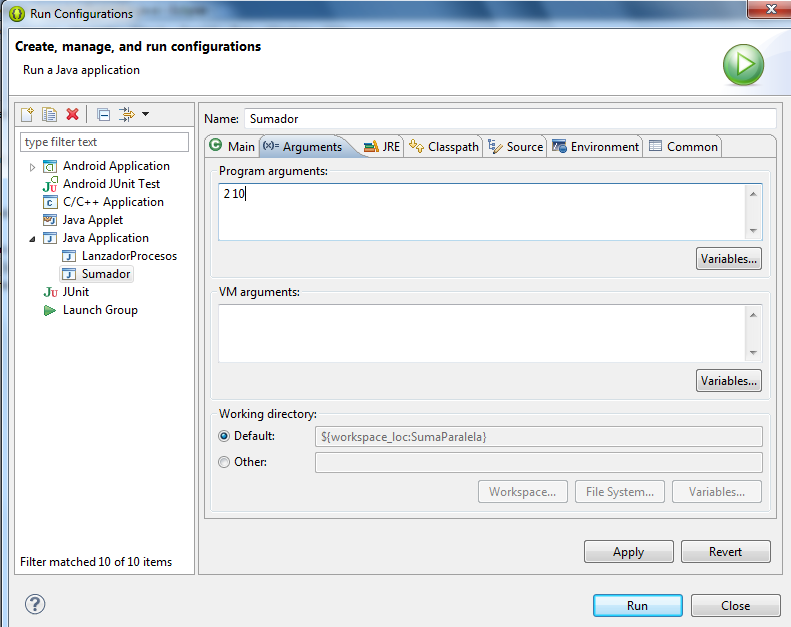
\includegraphics{configuraciones.png}
\caption{Modificando los argumentos del programa}\end{figure}

Una vez hecha la prueba de la clase sumador, le quitamos el main, y crearemos una clase que sea capaz de lanzar varios procesos. La clase \code{Sumador} se quedará así:

\begin{Verbatim}[commandchars=\\\{\}]
\PYG{k+kd}{public} \PYG{k+kd}{class} \PYG{n+nc}{Sumador} \PYG{o}{\PYGZob{}}
        \PYG{k+kd}{public} \PYG{k+kt}{int} \PYG{n+nf}{sumar}\PYG{o}{(}\PYG{k+kt}{int} \PYG{n}{n1}\PYG{o}{,} \PYG{k+kt}{int} \PYG{n}{n2}\PYG{o}{)}\PYG{o}{\PYGZob{}}
                \PYG{k+kt}{int} \PYG{n}{resultado}\PYG{o}{=}\PYG{l+m+mi}{0}\PYG{o}{;}
                \PYG{k}{for} \PYG{o}{(}\PYG{k+kt}{int} \PYG{n}{i}\PYG{o}{=}\PYG{n}{n1}\PYG{o}{;}\PYG{n}{i}\PYG{o}{\PYGZlt{}}\PYG{o}{=}\PYG{n}{n2}\PYG{o}{;}\PYG{n}{i}\PYG{o}{+}\PYG{o}{+}\PYG{o}{)}\PYG{o}{\PYGZob{}}
                        \PYG{n}{resultado}\PYG{o}{=}\PYG{n}{resultado}\PYG{o}{+}\PYG{n}{i}\PYG{o}{;}
                \PYG{o}{\PYGZcb{}}
                \PYG{k}{return} \PYG{n}{resultado}\PYG{o}{;}
        \PYG{o}{\PYGZcb{}}
\PYG{o}{\PYGZcb{}}
\end{Verbatim}

Y ahora tendremos una clase que lanza procesos de esta forma:

\begin{Verbatim}[commandchars=\\\{\}]
\PYG{k+kn}{package} \PYG{n}{com}\PYG{o}{.}\PYG{n+na}{ies}\PYG{o}{;}

\PYG{k+kd}{public} \PYG{k+kd}{class} \PYG{n+nc}{Lanzador} \PYG{o}{\PYGZob{}}
        \PYG{k+kd}{public} \PYG{k+kt}{void} \PYG{n+nf}{lanzarSumador}\PYG{o}{(}\PYG{n}{Integer} \PYG{n}{n1}\PYG{o}{,}
                        \PYG{n}{Integer} \PYG{n}{n2}\PYG{o}{)}\PYG{o}{\PYGZob{}}
                \PYG{n}{String} \PYG{n}{clase}\PYG{o}{=}\PYG{l+s}{\PYGZdq{}com.ies.Sumador\PYGZdq{}}\PYG{o}{;}
                \PYG{n}{ProcessBuilder} \PYG{n}{pb}\PYG{o}{;}
                \PYG{k}{try} \PYG{o}{\PYGZob{}}
                        \PYG{n}{pb} \PYG{o}{=} \PYG{k}{new} \PYG{n}{ProcessBuilder}\PYG{o}{(}
                                        \PYG{l+s}{\PYGZdq{}java\PYGZdq{}}\PYG{o}{,}\PYG{n}{clase}\PYG{o}{,}
                                        \PYG{n}{n1}\PYG{o}{.}\PYG{n+na}{toString}\PYG{o}{(}\PYG{o}{)}\PYG{o}{,}
                                        \PYG{n}{n2}\PYG{o}{.}\PYG{n+na}{toString}\PYG{o}{(}\PYG{o}{)}\PYG{o}{)}\PYG{o}{;}
                        \PYG{n}{pb}\PYG{o}{.}\PYG{n+na}{start}\PYG{o}{(}\PYG{o}{)}\PYG{o}{;}
                \PYG{o}{\PYGZcb{}} \PYG{k}{catch} \PYG{o}{(}\PYG{n}{Exception} \PYG{n}{e}\PYG{o}{)} \PYG{o}{\PYGZob{}}
                        \PYG{c+c1}{// TODO Auto\PYGZhy{}generated catch block}
                        \PYG{n}{e}\PYG{o}{.}\PYG{n+na}{printStackTrace}\PYG{o}{(}\PYG{o}{)}\PYG{o}{;}
                \PYG{o}{\PYGZcb{}}
        \PYG{o}{\PYGZcb{}}
        \PYG{k+kd}{public} \PYG{k+kd}{static} \PYG{k+kt}{void} \PYG{n+nf}{main}\PYG{o}{(}\PYG{n}{String}\PYG{o}{[}\PYG{o}{]} \PYG{n}{args}\PYG{o}{)}\PYG{o}{\PYGZob{}}
                \PYG{n}{Lanzador} \PYG{n}{l}\PYG{o}{=}\PYG{k}{new} \PYG{n}{Lanzador}\PYG{o}{(}\PYG{o}{)}\PYG{o}{;}
                \PYG{n}{l}\PYG{o}{.}\PYG{n+na}{lanzarSumador}\PYG{o}{(}\PYG{l+m+mi}{1}\PYG{o}{,} \PYG{l+m+mi}{51}\PYG{o}{)}\PYG{o}{;}
                \PYG{n}{l}\PYG{o}{.}\PYG{n+na}{lanzarSumador}\PYG{o}{(}\PYG{l+m+mi}{51}\PYG{o}{,} \PYG{l+m+mi}{100}\PYG{o}{)}\PYG{o}{;}
                \PYG{n}{System}\PYG{o}{.}\PYG{n+na}{out}\PYG{o}{.}\PYG{n+na}{println}\PYG{o}{(}\PYG{l+s}{\PYGZdq{}Ok\PYGZdq{}}\PYG{o}{)}\PYG{o}{;}
        \PYG{o}{\PYGZcb{}}
\PYG{o}{\PYGZcb{}}
\end{Verbatim}


\section{Comunicación entre procesos.}
\label{textos/tema1:comunicacion-entre-procesos}

\section{Gestión de procesos.}
\label{textos/tema1:gestion-de-procesos}

\section{Comandos para la gestión de procesos en sistemas libres y propietarios.}
\label{textos/tema1:comandos-para-la-gestion-de-procesos-en-sistemas-libres-y-propietarios}

\section{Sincronización entre procesos.}
\label{textos/tema1:sincronizacion-entre-procesos}

\section{Programación de aplicaciones multiproceso.}
\label{textos/tema1:programacion-de-aplicaciones-multiproceso}

\section{Documentación}
\label{textos/tema1:documentacion}

\section{Depuración.}
\label{textos/tema1:depuracion}

\chapter{Programación multihilo}
\label{textos/tema2:programacion-multihilo}\label{textos/tema2::doc}

\section{Recursos compartidos por los hilos.}
\label{textos/tema2:recursos-compartidos-por-los-hilos}

\section{Estados de un hilo. Cambios de estado.}
\label{textos/tema2:estados-de-un-hilo-cambios-de-estado}

\section{Elementos relacionados con la programación de hilos. Librerías y clases.}
\label{textos/tema2:elementos-relacionados-con-la-programacion-de-hilos-librerias-y-clases}

\section{Gestión de hilos.}
\label{textos/tema2:gestion-de-hilos}

\section{Creación, inicio y finalización.}
\label{textos/tema2:creacion-inicio-y-finalizacion}

\section{Sincronización de hilos.}
\label{textos/tema2:sincronizacion-de-hilos}

\section{Información entre hilos. Intercambio.}
\label{textos/tema2:informacion-entre-hilos-intercambio}

\section{Prioridades de los hilos.}
\label{textos/tema2:prioridades-de-los-hilos}

\section{Gestión de prioridades.}
\label{textos/tema2:gestion-de-prioridades}

\section{Compartición de información entre hilos.}
\label{textos/tema2:comparticion-de-informacion-entre-hilos}

\section{Programación de aplicaciones multihilo.}
\label{textos/tema2:programacion-de-aplicaciones-multihilo}

\section{Documentación.}
\label{textos/tema2:documentacion}

\section{Depuración.}
\label{textos/tema2:depuracion}

\chapter{Programación de comunicaciones en red}
\label{textos/tema3:programacion-de-comunicaciones-en-red}\label{textos/tema3::doc}

\section{Comunicación entre aplicaciones.}
\label{textos/tema3:comunicacion-entre-aplicaciones}

\section{Roles cliente y servidor.}
\label{textos/tema3:roles-cliente-y-servidor}

\section{Elementos de programación de aplicaciones en red. Librerías.}
\label{textos/tema3:elementos-de-programacion-de-aplicaciones-en-red-librerias}

\section{Funciones y objetos de las librerías.}
\label{textos/tema3:funciones-y-objetos-de-las-librerias}

\section{Sockets.}
\label{textos/tema3:sockets}

\section{Tipos de sockets. Características.}
\label{textos/tema3:tipos-de-sockets-caracteristicas}

\section{Creación de sockets.}
\label{textos/tema3:creacion-de-sockets}

\section{Enlazado y establecimiento de conexiones.}
\label{textos/tema3:enlazado-y-establecimiento-de-conexiones}

\section{Utilización de sockets para la transmisión y recepción de información.}
\label{textos/tema3:utilizacion-de-sockets-para-la-transmision-y-recepcion-de-informacion}

\section{Programación de aplicaciones cliente y servidor.}
\label{textos/tema3:programacion-de-aplicaciones-cliente-y-servidor}

\section{Utilización de hilos en la programación de aplicaciones en red.}
\label{textos/tema3:utilizacion-de-hilos-en-la-programacion-de-aplicaciones-en-red}

\section{Depuración.}
\label{textos/tema3:depuracion}

\chapter{Generación de servicios en red}
\label{textos/tema4:generacion-de-servicios-en-red}\label{textos/tema4::doc}

\section{Protocolos estándar de comunicación en red a nivel de aplicación}
\label{textos/tema4:protocolos-estandar-de-comunicacion-en-red-a-nivel-de-aplicacion}

\subsection{Telnet}
\label{textos/tema4:telnet}

\subsection{FTP}
\label{textos/tema4:ftp}

\subsection{HTTP}
\label{textos/tema4:http}

\subsection{POP3}
\label{textos/tema4:pop3}

\subsection{SMTP}
\label{textos/tema4:smtp}

\section{Librerías de clases y componentes.}
\label{textos/tema4:librerias-de-clases-y-componentes}

\section{Utilización de objetos predefinidos.}
\label{textos/tema4:utilizacion-de-objetos-predefinidos}

\section{Propiedades de los objetos predefinidos.}
\label{textos/tema4:propiedades-de-los-objetos-predefinidos}

\section{Métodos y eventos de los objetos predefinidos.}
\label{textos/tema4:metodos-y-eventos-de-los-objetos-predefinidos}

\section{Establecimiento y finalización de conexiones.}
\label{textos/tema4:establecimiento-y-finalizacion-de-conexiones}

\section{Transmisión de información.}
\label{textos/tema4:transmision-de-informacion}

\section{Programación de aplicaciones cliente.}
\label{textos/tema4:programacion-de-aplicaciones-cliente}

\section{Programación de servidores.}
\label{textos/tema4:programacion-de-servidores}

\section{Implementación de comunicaciones simultáneas.}
\label{textos/tema4:implementacion-de-comunicaciones-simultaneas}

\section{Documentación.}
\label{textos/tema4:documentacion}

\section{Depuración.}
\label{textos/tema4:depuracion}

\section{Monitorización de tiempos de respuesta.}
\label{textos/tema4:monitorizacion-de-tiempos-de-respuesta}

\chapter{Utilización de técnicas de programación segura}
\label{textos/tema5::doc}\label{textos/tema5:utilizacion-de-tecnicas-de-programacion-segura}

\section{Prácticas de programación segura.}
\label{textos/tema5:practicas-de-programacion-segura}

\section{Criptografía de clave pública y clave privada.}
\label{textos/tema5:criptografia-de-clave-publica-y-clave-privada}

\section{Principales aplicaciones de la criptografía.}
\label{textos/tema5:principales-aplicaciones-de-la-criptografia}

\section{Protocolos criptográficos.}
\label{textos/tema5:protocolos-criptograficos}

\section{Política de seguridad.}
\label{textos/tema5:politica-de-seguridad}

\section{Programación de mecanismos de control de acceso.}
\label{textos/tema5:programacion-de-mecanismos-de-control-de-acceso}

\section{Encriptación de información.}
\label{textos/tema5:encriptacion-de-informacion}

\section{Protocolos seguros de comunicaciones.}
\label{textos/tema5:protocolos-seguros-de-comunicaciones}

\section{Programación de aplicaciones con comunicaciones seguras.}
\label{textos/tema5:programacion-de-aplicaciones-con-comunicaciones-seguras}

\section{Pruebas y depuración.}
\label{textos/tema5:pruebas-y-depuracion}


\renewcommand{\indexname}{Índice}
\printindex
\end{document}
